\chapter{Preprocessing - Decaying the past and future}
\label{ch:preprocess}

\section{Motivations and methods}
For a system to predict motion it necessarily must encode some representation of time. 
%TODO reference some RNN and SNN papers...
Traditional approaches to this have been to design Recurrent Neural Networks (RNNs) or to use Spiking Neural Networks (SNNs). 
Many state-of-the-art learning learning techniques make the implicit assumption that time is discritised into the frame-rate of the camera used to make a recording. 
To leverage the existing literature and use these state-of-the-art models the event-based data must be converted into a representation that these networks can accept. 

\begin{wrapfigure}{r}{0.3\textwidth}
    \centering
    \label{fig:puppyBall}
    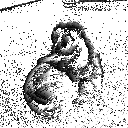
\includegraphics[width=0.3\textwidth]{puppyBall.png}
    \caption{A decayed image of a puppy with a ball}
\end{wrapfigure}
The simplest solution is to accumulate all the events in a given time slice into a 2D frame to recover images from the event-based data.
This is somewhat counter intuitive though as this forfeits all the temporal information which seperates the DVS from traditional cameras and results in a blury low resolution image. 
A method of preserving as much of the temporal information as possible is required. 


An approach to solve this problem is to choose a distinguished point in time, then construct a 2D image in which each pixels value is a function of its temporal distance to the distinguished point in time.
If only events that occured prior to the distiguished point in time are considered the resulting image would represent a faded history of what has just happened, this can be seen in figure \ref{fig:puppyBall} in which a recent history of the scene can be observed. 
Such images can be considered as a faded past, but are also known by many other equivilent names such as; temporal surface, decayed surface or time surface. 
There is no restriction as to why we must decay only into the past, a similarly interesting image can be produced decaying into the future from a distinguished point in time.
These decayed futures show where objects are moving to and can used as labels in a system trained to predict motion. 


The data is now in a form which can be used in traditional time-stepped neural networks and the temporal information has not been lost.
Still many questions remain to be explored such as what functions should be used to decay images and with what parameters.


\section{Function specifics and implementation}
%Include a quick maths wise description of this function\\
%Include some resulting images and discussion about each image as to why it is good or bad \\

The first and simplest decay function examined was linear decay. 
It can be characterised by equation \ref{eq:linearDecay}, intuitively in which the gradient (k) directly affects how much of the past (or future) is considered. 
Here $\Delta t$ is the temporal difference between the closest event for a given pixel and the distinguished point in time. 

% TODO why is this 1/k??

\begin{equation}
 \label{eq:linearDecay}
    f(\Delta t) = 
    \begin{cases}
    -\frac{1}{k}  \Delta t + 1 & 0\leq \Delta t \leq k \\
    0 & Otherwise
   \end{cases}
\end{equation}

An exponential function was also considered as a way to focus on only the most recent history.
Characterised by equation \ref{eq:expDecay} the length of history considered is dependent on the parameter k used. 

\begin{equation}
 \label{eq:expDecay}
    f(\Delta t) = exp\left(\frac{-\Delta t}{k}\right) \\
\end{equation}

To generate network inputs and outputs distinguished times must be selected and decayed around.
Each event in the event-stream could be used as a distinguished point and an input/output pair decayed around it.
This would generate a lot of redundant data as many similar events make up any given line.
Rather an event was selected at uniform time intervals to be decayed around.
A useful spacing was very problem dependent, interesting values to check were 10, 33 and 100 (\ms), unless otherwise specified 33\ms was used for this work so as to be similar to standard cameras. 
 


\subsection{Parameter influence}
Show some example parameters and how they affect the data \\


\section{Discussion}

 discuss the selections of k \\
 End up with a blur through time \\
 seems informative to humans at least? \\
 A little bit like a recurrent network (memory of past) \\
 Mention how training, validation and test datasets were generated.\\



